\documentclass{llncs}
\usepackage{amssymb}
\usepackage{url}
\usepackage{graphicx}

\title{Using Background Knowledge in GUHA Mining}
\author{Martin Ralbovsk\'{y}}
\institute{Department of Information and Knowledge Engineering,\\
University of Economics, Prague, W. Churchill Sq.~4, 130 67 Praha~3, Czech Republic
\\\email{martin.ralbovsky@gmail.com}}

\begin{document}
\maketitle

\begin{abstract}
Background knowledge can be used to enhance the data mining process. We discuss
the form of background knowledge suitable for data mining with the GUHA method.
A new formalization of background knowledge is presented and a tool for 
background knowledge rules validation is implemented in the Ferda system. We
test the new tool to validate rules from medical domain and discuss the usability
and possible improvements of the validation method. 
\end{abstract}

{\small {\bf Keywords:} Background knowledge, GUHA Method, Ferda}

\section{Introduction}
The GUHA method and procedures provide a powerful tool for knowledge discovery
in databases. However the comprehension of the method for non data mining
experts can be demanding. The experts in the domain need an instrument, which
can record their needs and present in to the data mining experts without 
knowing unnecessary details about mining techniques. \emph{Background knowledge}
rules as defined in this work can help to bridge the gap between the two 
players by defining data mining tasks. It can also help the data miners
to focus on the important relationships in the data and draw conclusions
about the data mining techniques.

The work is structured as follows: Section~\ref{section:guha} describes the
GUHA method, tools that implement the method and individual procedures used during
the work. Section~\ref{section:backgroundknowledge} describes the \emph{background
knowledge}, introduces new rule formalization and suggests usage of the formalization.
There are two experiments conducted in Section~\ref{section:mining} that use
\emph{background knowledge} rules to question the relevance of important quantifiers.
Finally, Section~\ref{section:related} puts the work into context of other works
dealing with \emph{background knowledge} and Section~\ref{section:conclusion} concludes
the work and gives ideas about future work.

\section{GUHA Method and Tools}
\label{section:guha}
\subsection{GUHA Method}
The GUHA (General Unary Hypotheses Automaton) is an original Czech method
of exploratory data analysis. Since the 60's, the method's theoretical 
frame (as described e.g. in \cite{GUHA1} or \cite{GUHA2}) was used over the
years as theoretical foundation for several data-mining tools. 

GUHA method is implemented by GUHA procedures. GUHA procedure is a program,
the input of which consists of the analyzed data and of a simple
definition of a large set of relevant patterns. The procedure automatically 
generates each particular pattern and verifies it against the analyzed data.
The output of the procedure consists of all patterns that are true in the
analyzed data and are not contained in other patterns.

\subsection{GUHA Tools} %nebo spis Tools Implementing GUHA Method - nevim
Apart from the tools presented in this section, several systems implementing
GUHA procedures were developed in the past. In recent years, the
\emph{LISp-Miner} system\footnote{See  \url{http://lispminer.vse.cz}.}
has been the most significant GUHA tool. This system
has been under development since 1996 at the University of Economics, Prague.
The system includes six GUHA procedures in addition to other data 
preparation and result interpretation modules. 

Although the \emph{LISp-Miner} proved to be a successful and stable system 
suitable for academic data mining, some functionality requirements occurred
that the system was not able to fulfill. These requirements concerned among others 
more coherent (and possibly visual) user environment or bigger modularity. 

In 2004, the Ferda project started as an initiative to build a new
visual data mining system that would eventually replace the
\emph{LISp-Miner} system. Creators (at the Faculty of Mathematics and Physics, 
Charles University, Prague) succeeded in developing an user friendly
visual system with advanced features such as high level modularity, support
for distributed computing or reusability of the task setting \cite{Ferda}.

The first version of Ferda (version 1.0 and 1.1) was still partly
dependent on the old \emph{LISp-Miner} system, because the task boxes
(visual elements in Ferda) used the \emph{LISp-Miner} hypotheses generation
engine and accessed it through the metabase layer. The new 2.0 version
is fully independent on the \emph{LISp-Miner} system and introduces a new
hypotheses generating engine with improved task setting abilities (details
can be found in \cite{Kuchar}). 

%\begin{figure}[h]
%\centering
%\mbox{\resizebox{0.95\textwidth}{!}{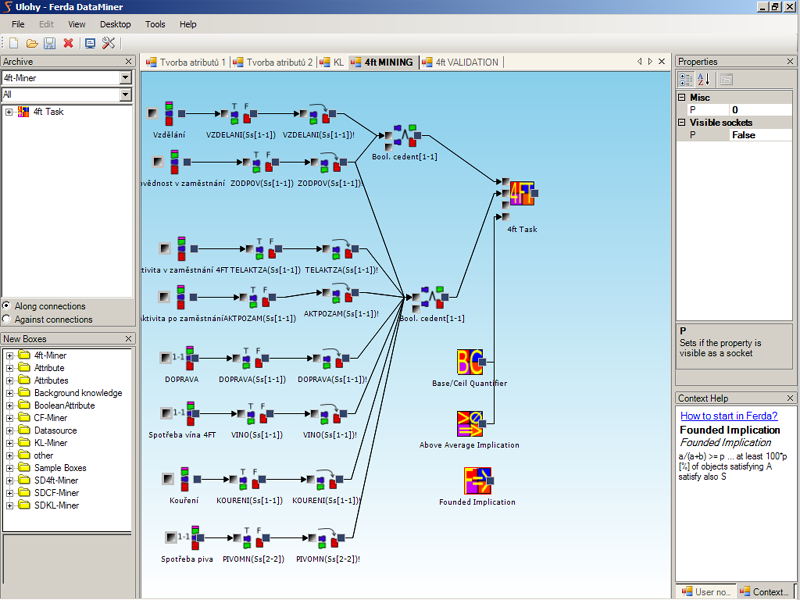
\includegraphics{ferda.png}}}
%\caption{The Ferda system}
%\label{fig:ferda}
%\end{figure}

Because of the advantages of the Ferda system, mainly the high level modularity
and the ability to incorporate new independent improvements into existing task
setup, we chose Ferda to be the implementation platform for this 
work\footnote{In the \emph{LISp-Miner} system, user has to build a standalone 
application above the existing metabase layer in order to add a module. In Ferda
user can add a box module that can take full advantage of partial results of
other boxes in the task. More details in \cite{Ferda}.}.

\subsection{Procedure 4FT}
One of the GUHA procedures used in this work is the \emph{4FT}
procedure\footnote{Note the terminological difference between 
the \emph{4FT} procedure and the \emph{4ft-Miner}. The \emph{4ft-Miner}
is a module of the \emph{LISp-Miner} system that implements the
\emph{4FT} GUHA procedure}. The procedure extends the historical
\emph{ASSOC} procedure for association rules mining and finds the rules
in form $\varphi \approx \psi / \chi$ where $\varphi$, $\psi$ and $\chi$ 
are \emph{boolean attributes} and $\approx$ is the \emph{4FT quantifier},
as defined in \cite{Kuchar} or \cite{Approach}. $\varphi$, $\psi$ and
$\chi$ are called \emph{antecedent}, \emph{succedent} and \emph{condition}
respectivelly\footnote{In other words, the procedure tests a condition
defined by \emph{4FT quantifier} over a four-fold table defined by
\emph{antecedent} and \emph{succedent} satisfiing conditing defined by
\emph{condition}}.

\subsection{Procedure KL}
\label{section:kl}
\emph{KL} is another GUHA procedure used in this work. The procedure mines
for hypotheses of form \emph{R} $\sim$ \emph{C}/$\chi$, where \emph{R} and
\emph{C} are \emph{categorial attributes} representing the row and column
attributes, $\sim$ is the \emph{KL quantifier} and $\chi$ is the \emph{boolean
attribute} representing condition (as defined in \cite{Kuchar} or \cite{KL}).

\section{Background Knowledge}
\label{section:backgroundknowledge}

\emph{Background knowledge} (or \emph{field knowledge}) is knowledge that
comes from the user or a community of users and integrates knowledge, which
the community can agree upon and consider it common. The term is vague and
different authors define \emph{background knowledge} differently (see 
Section~\ref{section:related} for details). In the context of GUHA mining,
we think of \emph{background knowledge} as a part of domain knowledge,
knowledge that is specific to particular domains (medicine, chemistry, etc.).
We define \emph{background knowledge} as a set of various verbal rules that
are accepted in a specific domain as a common knowledge. The rule can
define functional dependence between quantities, relationship between entities
or say something about their behavior.

\subsection{\emph{Background knowledge} examples}
\label{section:bkexamples}
Examples of such rules can be found in \cite{Diplomka}, where 46 rules from 
domains medicine and beer marketing were collected (\cite{Diplomka} is the primary
source material for this work). Below are presented example rules from the medical domain
\footnote{The rules were taken from the STULONG database. EUROMISE: The STULONG Project
\url{http://euromise.vse.cz/stulong/a-otazky/index.php?page=otazky}. The site is
available only in Czech.}:

\begin{itemize}
\item If education increases, wine consumption increases as well.
\item Patients with greater responsibility in work tend to drive to work by car.
\end{itemize}

Another type of rules displayed below can be found at the beer marketing domain. 
Unfortunately the source data from this domain are not available. Thus we 
cannot verify the rules against the source data (which will be done later).

\begin{itemize}
\item Younger consumers prefer draught beer.
\item Older consumers prefer beer in bottles.
\item Cheap brands are better sold in less economically developed regions.
\item More expensive brands are better sold during holidays.
\end{itemize}

\subsection{\emph{Background knowledge} usage}
Let us distinguish between two types of players present at the data mining process: 
the domain expert and the data miner. Then \emph{background knowledge} can be used
as an effective mean of communication between the two. 

The domain expert has extensive knowledge about the domain. He or she understands 
the meaning of entities or specific levels of measured quantities and can form 
general rules about behavior or relationships in the domain. Domain experts usually know
very little about data mining. On the other hand the data miner does not 
necessarily need to understand the complexity of the domain. The data miner understands
and knows how to use and interpret data mining technique(s).

The domain expert can form \emph{background knowledge} rules to specify what is
interesting or significant for him. The rules are passed to the data miner.
Each rule can be transformed into a mining task, which can be run on the examined
data afterwards. The results of one or more procedure's run (in the GUHA sense)
can confirm or disprove the rule on the examined data. Finding exceptions from a
given rule on given data pose also an interesting problem. The results from
the data miner can be at last summarized in the form of an analytical report and
returned back to the domain expert. All the usage possibilities stated above are
possible only with a sound formalization apparatus of \emph{background knowledge}
rules.

\section{Formalization of Background Knowledge}
\emph{Background knowledge} contains heterogeneous verbal formulations of dependences
and relationships in the domain. The relevance and validity of the formulations varies:
the relationships in physics are formed exactly by mathematical equations, but for
example in sociology they mean only expected behavior or opinion of a group of people.
Our aim is to find formalization usable for both domains.

\subsection{Qualitative Models}
\label{section:models}
In context of GUHA mining, this work (and the work \cite{Diplomka}) is the first
attempt to find suitable formalization of \emph{background knowledge} rules.
However, in \cite{Qualitative1} and \cite{Qualitative2} authors introduced
a formalization for induction learning based on qualitative models. 
We considered this model and found it not to be suitable for GUHA mining, mainly
because the strict mathematical requirements of the model. Details can be found
in \cite{Diplomka} in section 3.2.1.

\subsection{Attributes, Validation Literals and Abstract Quantifiers}
\label{section:formalization}
In order to continue efforts on using \emph{background knowledge} in GUHA
mining, we thought out a new formalization. The main idea of the new 
\emph{Formalization with attributes, validation literals and abstract quantifiers}
was to make the formalization as close to GUHA terms as possible while still 
enabling large expressing possibilities of the verbal rule\footnote{As was mentioned
in Section~\ref{section:backgroundknowledge} the overall theory containing all 
various types of \emph{background knowledge} does not exist. Therefore we can
define a \textbf{GUHA background knowledge} as yet another type of \emph{background
knowledge}.}. Because of short format of this article, we present only an overview
and an example of the new formalization with a little reasoning. The topic is fully
covered in \cite{Diplomka}, section 3.2.2.

%The new formalization is based on presumption that the correct \emph{attribute}
%creation is crutial for the whole data mining process\footnote{Attribute
%creation as described in \cite{Diplomka} or \cite{Kuchar} belongs to the \emph{Data
%preparation} phase of the CRISP-DM methodology.}. For example in some medical quantities
%(blood pressure, BMI) there are significant values defined that need to be taken into
%consideration during the \emph{attribute} creation phase - thresholds of high blood pressure
%or obesity levels of BMI. When the data miner creates a mistake in attribute creation,
%the mistake cannot me repaired in any subsequent phase and can lead to a wrong task
%setup.
\medskip
\emph{Attribute} is the basic term for the new formalization. \emph{Attribute}
is defined as a result of domain categorization\footnote{There are 4 different means
of categorization in the Ferda system, see \cite{Ferda} for details.} and is used
to create \emph{categorial attributes}, inputs of the \emph{KL} procedure. 

\medskip
\emph{Validation literal} is a special type of \emph{literal} used for the
\emph{background knowledge} validation. \emph{Literal} is a \emph{basic boolean 
attribute} or its negation. \emph{Basic boolean attribute} is defined by a non-empty subset
of the set of categories of an \emph{attribute}. We skip exact definitions, they
can be found in \cite{Kuchar} or \cite{Rauch}. We define the \emph{literal length}
as the size of the categories' subset. \emph{Validation literal} is a literal,
which has \emph{literal length} equal to 1.

\medskip
\emph{Abstract quantifier} is a generalization of a quantifier or quantifiers of 
a procedure (\emph{4FT} or \emph{KL}). The idea behind \emph{abstract quantifiers}
is to create a "black-box" quantifier: user does not need to fill any numeral 
parameters of the quantifier. The quantifier is then more suitable for transfering
verbal \emph{background knowledge} rules into formalized form.

\medskip
With all the terms explained, let us see how the formalization is applied to 
a specific verbal rule \texttt{If education increases, wine consumption increases as well.}
as presented in Section~\ref{section:bkexamples}. The rule defines relationship
between two measurable quantities of a pacient. These quantities are stored in the
database in the form of columns of a table, so \emph{attributes} can be created.
We name the attributes for \texttt{education} and \texttt{wine consumption}
\emph{education} and \emph{wine} respectivelly.

For this paragraph we will consider only the \emph{KL} procedure. From the 
Section~\ref{section:kl} the simplified form of hypotheses for \emph{KL}
\footnote{We do not consider the condition.} shortens to \emph{R} $\sim$ \emph{C} 
where \emph{R} and \emph{C} are \emph{categorial attributes}, which derive
from \emph{attributes}. When \texttt{education} and \texttt{wine consumption}
out of the rule are to be formalized with \emph{R} and \emph{C} of the hypothese,
then the part \texttt{If ... increases, ... increases as well} could be formalized with
a proper \emph{abstract quantifier}. In \cite{Diplomka} we called this quantifier
\emph{increasing dependence} and implemented it as a special setting of the 
\emph{Kendall quantifier}, as defined in \cite{KLKvant}. With all the knowledge
stated above, the rule \texttt{If education increases, wine consumption increases
as well} can be formally written as \emph{education} $\uparrow$ \emph{wine}, where
$\uparrow$ states for \emph{increasing dependence abstract quantifier}.

We can also define the formalization for the \emph{4FT} procedure. The hypotheses
of this procedure consist of \emph{boolean attributes}, therefore \emph{validation
literals} need to be used. If we presume correct categorization, out of
\emph{attributes education} and \emph{wine} the \emph{validation literals
education(HIGH)} and \emph{wine(HIGH)} can be created\footnote{\emph{Validation
literal} allows sign setting. Here both signs are \emph{positive}.}. Similarly
to \emph{KL} formalization we can use \emph{abstract quantifier} to 
note the dependence. Then the rule \texttt{If education increases, wine consumption
increases as well} can be formalized as \emph{education(HIGH)} $\Rightarrow$
\emph{wine(HIGH)} with a proper \emph{abstract quantifier} $\Rightarrow$\footnote{
Formalization with the \emph{4FT} procedure does not consider the whole \emph{attributes}
but only some categories, thus it is weaker. However there may be situations 
when it is feasible to use the \emph{4FT} procedure. Details are discussed in
\cite{Diplomka}, Section 3.2.2.}. 

In the beginning of this section, a requirement was given on the formalization
to be able to represent various kinds of relationships between the
entities of the domain. The \emph{formalization with attributes, validation 
literals and abstract quantifiers} clearly fulfills this requirement, because the
formalization does not pose any restrictions on the relationships - 
the relationship is expressed by the \emph{abstract quantifier}. 

\emph{Background knowledge} rule was defined in Section~\ref{section:backgroundknowledge}
as verbal rule declared by the domain expert. Obviously, not all the rules formed in natural
language can be formalized by the formalization we created. Despite this, we think that
a substantial part of all the interesting rules can be formalized and the rest could be
very hardly analyzed by the implemented GUHA procedures\footnote{\emph{4FT} and \emph{KL}}
anyway. Below a template for verbal rules that can be formalized is presented:

\medskip
\textbf{Under a certain condition defined by a set of \emph{validation literals},
two quantities, entities or states, defined by sets of \emph{validation literals}
or \emph{attributes} are in a \emph{relationship}. The relationship is defined by
the \emph{abstract quantifier}.}

\medskip
Number of verbal rules that match with the template is high, note also that all
the rules presented in Section~\ref{section:bkexamples} match with the template.
This fact itself does not assure success of the formalization, mainly because the
real weakness (and strength as well) lies in definition of sound\emph{abstract
quantifiers}. We will discuss this matter more in Section~\ref{section:mining}

\section{Experience with Background Knowledge aided GUHA mining}
\label{section:mining}

\subsection{Implemented \emph{backroung knowledge} validation tool in Ferda system}
A tool for \emph{background knowledge} validation was implemented in the Ferda system for
purposes of this work and of work \cite{Diplomka}.
The tool consist of 10 new box modules that include validation boxes, and boxes enabling
the \emph{formalization with attributes, validation literals and abstract quantifiers}
construction\footnote{Because the Ferda version 2.0 was still in the development at
the time \emph{background knowledge} validation was implemented, we used the version 1.0 
We plan to develop the tool also for the version 2.0, with improved possibilities that
this version enables.}.
The details of the implementation, with proper explanation of the modules
and description of validation algorithms can be found in \cite{Diplomka}.

Alhough the implementation details of the tool were skipped because of the short 
format of the article, let us mention the implemented \emph{abstract quantifiers}.
For the \emph{KL} procedure, we implemented the \emph{Increasing dependence} and
the \emph{Decreasing dependence abstract quantifiers}. As mentioned before, 
these quantifiers are defined as special settings of the \emph{Kendall quantifier}.
For the \emph{4FT} procedure, there exist formal classes of quantifiers and each
quantifier belongs to one of that classes\cite{Classes}. Therefore we chose the
\emph{abstract quantifiers} to represent each of the classes. User that has the
knowledge of particular quantifiers -- does not need the blackbox model (see 
Section~\ref{section:formalization}), can also validate the background knowledge
with the normal quantifiers\footnote{More details on the topic in 
\cite{Diplomka}.}.

\subsection{Validated rules}
Out of the 46 gathered \emph{background knowledge} rules, we chose 8 rules for
validation from the medical domain\footnote{We chose the medical domain, because
the source data exist. The rules were selected as a sample of the rules that can
be mined upon (without changing the database schema).}. Rules are listed in Table
 \ref{tab:rules}. 

\begin{table}[h]
	\centering
	\begin{tabular}{|p{2cm}|p{4cm}|p{4cm}|}
		\hline
			\textbf{Number} & \textbf{Rule} & \\
		\hline
			\textbf{1} & If education increases & physical activity after work increases as well\\
		\hline
			\textbf{2} & If education increases & responsibility in work increases as well\\
		\hline
			\textbf{3} & If education increases & wine consumption increases as well\\
		\hline
			\textbf{4} & If education increases & smoking decreases\\
		\hline
			\textbf{5} & If education increases & physical activity in work decreases\\
		\hline
			\textbf{6} & If education increases & beer consumption decreases\\
		\hline
			\textbf{7} & Patients with greater responsibility in work & tend to drive to work by car\\
		\hline
			\textbf{8} & Patients with smaller responsibility in work & tend to use public transpor to
			get to work\\
		\hline
	\end{tabular}
\caption{Validated rules}
\label{tab:rules}
\end{table}

\subsection{Validation with default quantifiers' settings}
There are treshold values of parameters defined for each quantifier, which tell
us when quantifier's output is significant. We call them \emph{default quantifiers'
settings}. These values were set up by an agreement among data mining experts.
The first conducted experiment was to verify the values with the aid of the rule
validation on the STULONG source data.

For the \emph{KL} procedure \emph{abstract quantifiers}, we chose the 
\emph{increasing} and \emph{decreasing dependece} with settings of 0.7
and -0.7 value of the \emph{Kendall's} $\tau_{b}$ parameter\footnote{Explanation
in \cite{Diplomka}, Section 5.3.5.}. For the \emph{4FT} procedure, we wanted
to examine settings of the two most used quantifiers from the history of the procedure:
the \emph{founded implication} and the \emph{above average} quantifiers. For the
\emph{founded implication} quantifier, the default values are 0.95 for the
\emph{P} parameter and 0.05 for the \emph{base} parameter. For the \emph{above
average} quantifier, the default values are 1.2 for the \emph{P} parameter
and 0.05 for the \emph{Base} parameter\footnote{as defined in \cite{Classes}}. 
The \emph{founded implication} and \emph{above average} quantifiers and their
default settings are stored in the \emph{Implication} and \emph{Other abstract
quantifiers}\footnote{In the implemented tool of the Ferda system}, respectivelly.

\begin{table}[h]
	\centering
	\begin{tabular}{|p{2,5cm}|p{1cm}|p{1cm}|p{1cm}|p{1cm}|}
		\hline
		\textbf{Rule number}&\textbf{ID}&\textbf{DD}&\textbf{FI}&\textbf{AA}\\
		\hline
		1&YES&x&NO&NO\\
		\hline
		2&YES&x&NO&NO\\
		\hline
		3&NO&x&YES&NO\\
		\hline
		4&x&NO&NO&NO\\
		\hline
		5&x&NO&NO&YES\\
		\hline
		6&x&NO&NO&NO\\
		\hline
		7&x&x&NO&NO\\
		\hline
		8&x&x&NO&NO\\
		\hline
	\end{tabular}
\caption{Validation of quantifier's settings}
\label{tab:validation1}
\end{table}

The Table~\ref{tab:validation1} shows the results of the first experiment. The \textbf{ID},
\textbf{DD}, \textbf{FI} and \textbf{AA} stands for \emph{increasing dependence}, 
\emph{decreasing dependence}, \emph{founded implication} and \emph{above average}
quantifiers. \textbf{YES} means that the rule was validated with the given quantifier,
\textbf{NO} means that the rule was not validated and \textbf{x} means that the
rule was not meaningful for given quantifier.

Before we draw any conclusions from the experiment, let us first state some 
presumptions about the data source. The data table \emph{entry}, which was mined 
upon, contains records about the entry examination of 1417 patients. Because of
this number, we consider the data to be statistically significant. We also
presume no errors in the data and proper categorization (described in \cite{Diplomka}). 
Finally, when we want to question settings of individual quantifiers, we
presume that the \emph{field knowledge} rules are "somehow stored" in the data. 

The most interesting result of the experiment the disapproval of all the rules except
one with the \emph{founded implication} and also the \emph{above average}
quantifier. If a data miner uses the \emph{founded implication} of \emph{above
average} quantifiers or derived \emph{abstract quantifiers} with default settings,
he probably will not validate any rules - the default settings are too restrictive.

\subsection{Finding suitable quantifiers' settings}
As the previous section showed, the default settings of a quantifier can be
misleading. The next conducted experiment tries to find suitable quantifiers'
settings, based on the \emph{background knowledge} rule validation. We gradually
decreased the \emph{P} settings of the \emph{founded implication} and
\emph{above average} quantifiers. We did not experiment with the
\emph{KL} quantifiers, because of the complexity of the procedure\footnote{The 
results need not to improve merely by changing a parameter of a quantifier. 
We also need to take the shape of the \emph{KL} contingency table into consideration.}.
With this technique, we could examine more \emph{background knowledge} rules,
determine the value of the parameter for each rule and compute the average
of the values. This average value could be used in new mining to discover
new relationships in the data.

New mining with the quantifier can be done with this average
value that could discover new relationships in the data.

\begin{table}[h]
	\centering
	\begin{tabular}{|p{2,5cm}|p{1,5cm}|p{1,5cm}|}
		\hline
		\textbf{Rule number}&\textbf{FI}&\textbf{AA}\\
		\hline
		1&0.83&1,03\\
		\hline
		2&0.72&0.43\\
		\hline
		3&1&0.68\\
		\hline
		4&0.32&1.17\\
		\hline
		5&0.28&1.34\\
		\hline
		6&0.38&1.17\\
		\hline
		7&0.16&1.15\\
		\hline
		8&0.64&1.07\\
		\hline
	\end{tabular}
\caption{Exact quantifiers values}
\label{tab:validation2}
\end{table}

As we can see in Table~\ref{tab:validation2}, the results of the experiment
are rather dissapointing. For the \emph{founded implication} quantifier, majority
of rules had the \emph{P} value below 0.5. This means that we cannot rely on
the quantifier when validating. We got better results for the \emph{above average}
quantifier where the \emph{P} parameter was only twice below 1. However, only once
the value exceeded the desired 1.2 value. 

To summarize, the experiments with \emph{abstract quantifiers} based on the 
\emph{founded implication} and the \emph{above average} quantifiers were not 
successful. These quantifiers have been used as pivot quantifiers for the \emph{4FT}
mining. However, as our experiments showed, they failed to validate \emph{background
rules} which, according to presumption we made, should be present in the data. 
Other absract quantifiers should be developed and used in order to get better
validation results. The Section~\ref{section:related} introduces works that
should deal with the topic. 

\section{Related work}
\label{section:related}

As was mentioned in Section~\ref{section:models}, there have been other attempts
in the past to formalize \emph{background knowledge}, described in \cite{Qualitative1}
and \cite{Qualitative2}. However, this formalization was no use for GUHA mining. 

In \cite{Puppe}, authors use \emph{background knowledge} for subgroup discovery.
Improtant part of the work tries to divide \emph{background knowledge} into classes and deals
separately with each class. Unfortunatelly the rules and formalization defined in
this work do not belong to any of the classes defined.

Treti clanek ziskat od Svatka. 

\section{Conclusion and Future Work}
\label{section:conclusion}

The work presents an innovative look on \emph{background knowledge} in the context
of GUHA mining. We found techniques to enhance the cooperation between domain expert
and the data miner. In order to carry out the techniques, new 
\emph{formalization with attributes, validation literals and abstract quantifiers}
of the \emph{background knowledge} rules was invented. This formalization suits
especially the GUHA procedures implemented in the Ferda system.

After implementing a tool for rule validation in the Ferda system, we formalized
rules from the medical domain and used them to question the relevance of quantifiers'
settings in of the \emph{KL} and \emph{4FT} procedure. Two conducted experiments
showed clear inaccuracy in validation of individual rules and a further need to
improve the understanding of the quantifiers and their usage. 

There are two main directions for future work in the field. The first one covers
further investigation of \emph{abstract quantifiers} and conditions under they
can be used. New \emph{abstract quantifiers} should be defined, which would have
better support of the \emph{field knowledge} rules presented by the domain experts.
\cite{Kupka} should be a work on this topic. The second direction is the further
improvement of interaction between the data miner and the domain expert. Automated
tool should be developed to collect, store and formalize the \emph{background
knowledge} rules. In further future, there is a need for automated task generation
and result interpretation based on the rules. The \emph{Ever-Miner} system 
aims to realize these plans\footnote{Plans to implement the \emph{Ever-Miner} system
are described in \cite{Diplomka}}. 

\begin{thebibliography}{20}

\bibitem{Puppe}
Atzmueller M., Puppe F.: \emph{A Methodological View on Knowledge-Intensive Subgroup
Discovery}. In... tady dopsat odkud to je.

\bibitem{Qualitative1}
Clark P., Matwin S.: \emph{Using Qualitative Models to Guide Inductive Learning}.
In: Proceedings 10$^{th}$ International Machine Learning Conference (ML93), pg. 
49 - 56

\bibitem{GUHA1}
H\'{a}jek P., Havel I., Chytil M.: \emph{The GUHA method of
automatic hypotheses determination}. Computing 1, 1966, p. 293 -- 308

\bibitem{GUHA2}
H\'{a}jek P., Havr\'{a}nek, T.: \emph{Mechanising Hypothesis
Formation - Mathematical  Foundations  for  a   General  Theory}.
Springer-Verlag: Berlin  - Heidelberg - New York, 1978.

\bibitem{Ferda}
Kov\'{a}\v{c} M., Kucha\v{r} T., Kuzmin A., Ralbovsk\'{y} M.: \emph{Ferda, 
New Visual Environment for Data Mining}. Znalosti 2006, 
Conference on Data Mining, Hradec Kr\'{a}lov\'{e} 2006,p.~118~--~129 (in Czech)

\bibitem{Kuchar}
Kucha\v{r} T.: \emph{Experimental GUHA Procedures}, Master Thesis, 
Faculty of Mathematics and Physics, Charles University, Prague 2006 (in Czech)

\bibitem{Kupka}
Kupka D.: \emph{User support 4ft-Miner procedure for Data Mining}. Master Thesis,
Faculty of Mathematics and Physics, Charles University, Prague 2006 (in Czech)

\bibitem{KLKvant}
L\'{i}n V.: \emph{053 Definition of KL quantifiers}. LISp-Miner system documentation
(in Czech)

\bibitem{Qualitative2}
Matwin S., Rouge T.: \emph{Explainable Induction with an Imperfect Qualitative Model}.
\url{http://citeseer.ist.psu.edu/matwin95explainable.html}

\bibitem{Classes}
Rauch J.: \emph{Classes of Association Rules - an Overview}. In: Lin T. Y. (ed): 
Foundations of Semantic Oriented Data and Web Mining. Proceedings of a workshop
held in conjunction with 2005 IEEE International Conference on Data Minig

\bibitem{Rauch}
Rauch J.: \emph{Logic of Association Rules}. In: Applied Inteligence, Vol. 22,
Issue 1, p.~9~--~28

\bibitem{Approach}
Rauch, J., \v{S}im\accent23unek, M.: \emph{An Alternative Approach to Mining
Association Rules}. In: Lin T. Y., Ohsuga S., Liau C. J., Tsumomo S. (eds.),
Data Mining: Foundations, Methods, and Applications, Springer-Verlag, 2005

\bibitem{KL}
Rauch, J., \v{S}im\accent23unek, M.: \emph{Mining for Patterns Based on 
Contingency Tables by KL-Miner - First Experience}. In: ICDM2003 Workshop
\emph{Foundations and New Directions of Data Mining}, \url{http://www.cs.uvm.edu/~xwu/icdm-03.html}

\bibitem{Diplomka}
Ralbovsk\'{y} M.: \emph{Usage of Domain Knowledge for Applications of GUHA
Procedures}, Master Thesis, Faculty of Mathematics and Physics, Charles University,
Prague 2006 (in Czech)

\bibitem{Ontology}
Sv\'{a}tek V., Rauch J., Ralbovsk\'{y} M.: \emph{Ontology-Enhanced Association
Mining}. In: Ackermann, Berendt (eds.). Semantics, Web and Mining, 
Springer-Verlag, 2006

\end{thebibliography}

\end{document}